\documentclass{article}

\begin{document}


\setlength{\parindent}{6ex}

\begin{figure}
    \centering
    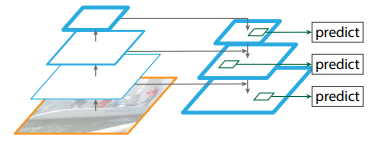
\includegraphics[width=\textwidth]{fpnvis}
    \caption{FPN Architecture}
    \label{fig:fpnvis1}
\end{figure}

\indent

Multi-scale handling is mentioned in section 2.3. For multi-scale input images, 
the required time and memory is too high to be trained end-to-end simultaneously. 
Also, pyramidal feature hiearchy in figure \ref{fig:multiscalefeatmaps1} is not 
effective for accurate object detection, specifically in small objects due to the 
resolution of feature maps. Feature Pyramid Network (FPN) is designed as a 
feature extractor keeping accuracy and speed in mind. \par 

As you can see in figure \ref{fig:fpnvis1}, FPN consists of a bottom-up and 
top-down pathway. In the bottom-up pathway, as in pyramidal feature hiearchy 
(Fig. \ref{fig:fig:multiscalefeatmaps1}(c)), a convolutional network is used as 
feature extractor. 
 
\end{document}